\chapter{Registri a scorrimento e contatori}
\label{ch:registri-contatori}
\textit{(17 aprile 2026)}

% ======================================================================
\section{Registri a scorrimento}

Un \textbf{registro a scorrimento} (shift register) è una catena di Flip-Flop di tipo D collegati in serie: l'uscita $Q$ di ciascuno è collegata all'ingresso $D$ del successivo. Ad ogni fronte di clock, ogni Flip-Flop «passa» il proprio valore al vicino di destra, come in un nastro trasportatore. In questo modo il dato si \emph{sposta} di una posizione ad ogni colpo di clock.

\vspace{2mm}
\noindent Per chiarire con un esempio: se il registro contiene i bit $[X, Y, Z]$ e arriva un nuovo dato $W$ dall'ingresso, dopo un tick di clock il contenuto diventa $[W, X, Y]$: il vecchio $Z$ è uscito, $X$ e $Y$ sono slittati di una posizione, e il nuovo $W$ è entrato in testa.

\subsection{Modalità di trasmissione dati}

A seconda di come si alimentano i dati in ingresso e di come si leggono in uscita, lo stesso registro fisico può funzionare in quattro modalità distinte:

\begin{itemize}[leftmargin=1.5em]
    \item \textbf{SISO} (Serial In -- Serial Out): il dato entra un bit alla volta dall'ingresso seriale ed esce un bit alla volta dall'ultimo FF. Utilizzo principale: \textbf{ritardare} un segnale digitale di esattamente $n$ cicli di clock.
    \item \textbf{SIPO} (Serial In -- Parallel Out): il dato entra un bit alla volta, ma si leggono in uscita \emph{contemporaneamente} tutti i bit memorizzati. Utilizzo tipico: convertire una trasmissione seriale (es. linea RS-232) in un dato parallelo leggibile dalla CPU.
    \item \textbf{PISO} (Parallel In -- Serial Out): si caricano tutti i bit in un solo colpo (caricamento parallelo), poi li si trasmette uno alla volta. Utilizzo: serializzare un dato parallelo per inviarlo su un bus seriale.
    \item \textbf{PIPO} (Parallel In -- Parallel Out): caricamento parallelo e lettura parallela. Funziona come un \textbf{registro di memoria}: cattura uno snapshot di un dato a $n$ bit e lo mantiene in uscita fino al prossimo aggiornamento.
\end{itemize}

\subsection{Temporizzazione e vincoli}

Affinché il registro funzioni correttamente, il clock deve rispettare due vincoli temporali critici propri di ogni Flip-Flop:

\begin{important}
$T_P > T_H$, \quad $T_S + T_P < T_{CLK}$

\begin{itemize}[leftmargin=1.3em]
  \item $T_{setup}$ ($T_S$): il dato deve essere stabile sull'ingresso $D$ per almeno questo tempo \emph{prima} del fronte di clock, altrimenti non viene catturato correttamente.
  \item $T_{hold}$ ($T_H$): il dato deve rimanere stabile per almeno questo tempo \emph{dopo} il fronte di clock.
  \item $T_P$: tempo di propagazione attraverso il FF (quanto ci vuole affinché, dopo il fronte, l'uscita $Q$ si aggiorni e il nuovo valore sia pronto per il FF successivo).
  \item $I_N = D_{SR}$: dato seriale in ingresso al registro.
\end{itemize}
\end{important}

\noindent In parole semplici: il periodo del clock deve essere abbastanza lungo da permettere al segnale di attraversare il FF e di stabilizzarsi sul $D$ del successivo \emph{prima} che arrivi il fronte successivo. Se il clock è troppo veloce si leggono valori errati.

\medskip
\noindent Nei registri a scorrimento sono presenti i seguenti segnali di controllo:
\begin{itemize}[leftmargin=1.5em]
    \item \textbf{CLK}: sincronizza ogni scorrimento.
    \item \textbf{RESET/CLEAR}: azzera immediatamente l'intero registro.
    \item \textbf{SET}: forza l'uscita a $1$ (preset).
    \item \textbf{ENABLE}: quando basso, congela il registro bloccando gli scorrimenti.
\end{itemize}

\medskip
\noindent\textcolor{teal}{\textbf{Riassunto -- Differenza tra registro normale e registro a scorrimento:}}
\begin{itemize}[leftmargin=1.5em]
    \item \textbf{Registro normale (PIPO)}: cattura e conserva un dato multi-bit aggiornandolo in blocco. Non c'è scorrimento interno.
    \item \textbf{Registro a scorrimento}: conserva il dato \emph{e lo fa scorrere} di una posizione ad ogni clock, abilitando la conversione seriale$\leftrightarrow$parallelo e il ritardo digitale.
\end{itemize}

\subsection{Schemi dei registri (PIPO, SISO, SIPO, PISO)}

Di seguito sono riportati gli schemi a blocchi semplificati delle quattro configurazioni
(ogni blocco è un FF-D con ingresso $D$, uscita $Q$, ingresso di clock e ingressi asincroni
$S$ di set e $R$ di reset). Nel PISO un multiplexer sceglie, tramite il segnale
Shift/$\overline{\text{Load}}$, se il secondo flip-flop riceve il bit del flip-flop precedente
(shift, ingresso 1) oppure il dato parallelo $P_1$ (caricamento, ingresso 0).

\begin{figure}[H]
\centering
\begin{circuitikz}[scale=0.9, every node/.style={scale=0.9}, line width=0.8pt]
\tikzset{
  mypipo/.style={flipflop, flipflop def={t1=$D_0$, t6=$Q_0$, c2=1}},
  mypipo1/.style={flipflop, flipflop def={t1=$D_1$, t6=$Q_1$, c2=1}},
  mysiso0/.style={flipflop, flipflop def={t1=$D_0$, t6=$Q_0$, c2=1}},
  mysiso1/.style={flipflop, flipflop def={t1=$D_1$, t6=$Q_1$, c2=1}}
}

% ======== TOP ROW ========

% -------- PIPO --------
\begin{scope}[yshift=0cm]
\node[mypipo] (FF0) at (0,3.0) {};
\node[mypipo1] (FF1) at (0,0) {};

\draw (FF0.pin 1) ++(-1.0,0) -- (FF0.pin 1);
\draw (FF1.pin 1) ++(-1.0,0) -- (FF1.pin 1);
\draw (FF0.pin 6) -- ++(1.0,0);
\draw (FF1.pin 6) -- ++(1.0,0);

% CLK
\coordinate (clkstart) at (-2.5, -1.2);
\coordinate (cb1) at (-1.5, -1.2);
\draw (clkstart) node[left, font=\bfseries, text=blue!60!black] {CLK} -- (cb1);
\draw (cb1) -- (cb1 |- FF1.pin 2) -- (FF1.pin 2);
\draw (cb1 |- FF1.pin 2) node[circle,fill,inner sep=1.2pt]{} -- (cb1 |- FF0.pin 2) -- (FF0.pin 2);

\node[font=\Large\bfseries, text=black] at (0,-2.2) {PIPO};
\end{scope}

% -------- SISO --------
\begin{scope}[xshift=9cm]
\node[mysiso0] (FF0) at (0,1.25) {};
\node[mysiso1] (FF1) at (3.5,1.25) {};

\draw (FF0.pin 1) ++(-1.0,0) -- (FF0.pin 1);
\draw (FF1.pin 6) -- ++(1.0,0);

\draw (FF0.pin 6) -- ++(0.7,0) coordinate (q0_bot) -- (q0_bot |- FF1.pin 1) coordinate (q0_top) -- (FF1.pin 1);

\draw (FF0.north) -- (FF0.north |- 0,2.75) node[above, font=\small\bfseries] {S};
\draw (FF1.north) -- (FF1.north |- 0,2.75) node[above, font=\small\bfseries] {S};
\draw (FF0.south) -- (FF0.south |- 0,-0.2) node[below, font=\small\bfseries] {R};
\draw (FF1.south) -- (FF1.south |- 0,-0.2) node[below, font=\small\bfseries] {R};

% CLK
\coordinate (clkstart) at (-2.5, -1.0);
\coordinate (cb0) at (-1.5, -1.0);
\coordinate (cb1) at (2.0, -1.0);
\draw (clkstart) node[left, font=\bfseries, text=blue!60!black] {CLK} -- (cb1);
\draw (cb0) -- (cb0 |- FF0.pin 2) -- (FF0.pin 2);
\draw (cb1) -- (cb1 |- FF1.pin 2) -- (FF1.pin 2);

\node[font=\Large\bfseries, text=black] at (1.75,-2.2) {SISO};
\end{scope}

% ======== BOTTOM ROW ========

% -------- SIPO --------
\begin{scope}[yshift=-8cm]
\node[mysiso0] (FF0) at (0,1.25) {};
\node[mysiso1] (FF1) at (3.5,1.25) {};

\draw (FF0.pin 1) ++(-1.0,0) -- (FF0.pin 1);
\draw (FF0.pin 6) -- ++(0.7,0) coordinate (q0_bot) -- (q0_bot |- FF1.pin 1) coordinate (q0_top) -- (FF1.pin 1);
\draw (FF1.pin 6) -- ++(0.7,0) coordinate (q1_bot);

\draw (FF0.north) -- (FF0.north |- 0,2.75) node[above, font=\small\bfseries] {S};
\draw (FF1.north) -- (FF1.north |- 0,2.75) node[above, font=\small\bfseries] {S};
\draw (FF0.south) -- (FF0.south |- 0,-0.2) node[below, font=\small\bfseries] {R};
\draw (FF1.south) -- (FF1.south |- 0,-0.2) node[below, font=\small\bfseries] {R};

% SIPO outputs
\draw (q0_top) node[circle, fill, inner sep=1.2pt] {} -- ++(0, 1.0);
\draw (q1_bot) node[circle, fill, inner sep=1.2pt] {} -- ++(0, 1.0);

% CLK
\coordinate (clkstart) at (-2.5, -1.0);
\coordinate (cb0) at (-1.5, -1.0);
\coordinate (cb1) at (2.0, -1.0);
\draw (clkstart) node[left, font=\bfseries, text=blue!60!black] {CLK} -- (cb1);
\draw (cb0) -- (cb0 |- FF0.pin 2) -- (FF0.pin 2);
\draw (cb1) -- (cb1 |- FF1.pin 2) -- (FF1.pin 2);

\node[font=\Large\bfseries, text=black] at (1.75,-2.2) {SIPO};
\end{scope}

% -------- PISO --------
\begin{scope}[xshift=9cm, yshift=-8cm]
\node[mysiso0] (FF0) at (0,1.25) {};
\node[mysiso1] (FF1) at (4.6,1.25) {};

\draw (FF0.north) -- (FF0.north |- 0,2.85) node[above, font=\small\bfseries] {S};
\draw (FF1.north) -- (FF1.north |- 0,2.85) node[above, font=\small\bfseries] {S};
\draw (FF0.south) -- (FF0.south |- 0,-0.3) node[below, font=\small\bfseries] {R};
\draw (FF1.south) -- (FF1.south |- 0,-0.3) node[below, font=\small\bfseries] {R};

% MUX block
\path (FF1.pin 1) ++(-0.6,0) node[draw, fill=gray!20, minimum height=0.9cm, minimum width=0.6cm, anchor=east] (mux) {\scriptsize MUX};

% Ingresso parallelo P0
\draw (FF0.pin 1 |- 0,2.85) ++(-0.6,0) coordinate (p0_start) node[above, font=\small\bfseries] {$P_0$};
\draw[->] (p0_start) |- (FF0.pin 1);

% Ingresso seriale Q0 -> ingresso 0 del MUX
\draw (FF0.pin 6) -- ++(0.5,0) |- ([yshift=-8pt]mux.west) node[left, font=\tiny] {1};

% Ingresso parallelo P1 -> ingresso 1 del MUX
\draw ([yshift=8pt]mux.west |- 0,2.85) ++(-0.4,0) coordinate (p1_start) node[above, font=\small\bfseries] {$P_1$};
\draw[->] (p1_start) |- ([yshift=8pt]mux.west) node[left, font=\tiny] {0};

\draw (mux.east) -- (FF1.pin 1);
\draw (FF1.pin 6) -- ++(1.0,0);

% Linea di selezione dal basso
\draw[<-, thick, gray!70!black] (mux.south) -- ++(0,-0.6) node[below, font=\scriptsize\bfseries, text=gray!80!black] {Shift/$\overline{\text{Load}}$};

% CLK
\coordinate (clkstart) at (-2.5, -1.0);
\coordinate (cb0) at (-1.5, -1.0);
\coordinate (cb1) at (2.6, -1.0);
\draw (clkstart) node[left, font=\bfseries, text=blue!60!black] {CLK} -- (cb1);
\draw (cb0) -- (cb0 |- FF0.pin 2) -- (FF0.pin 2);
\draw (cb1) -- (cb1 |- FF1.pin 2) -- (FF1.pin 2);

\node[font=\Large\bfseries, text=black] at (2.3,-2.2) {PISO};
\end{scope}

\end{circuitikz}
\caption{Schemi a blocchi dei registri a scorrimento: PIPO, SISO, SIPO, e PISO.}
\end{figure}

% ======================================================================
\section{Contatori}
\textit{(17 aprile 2026)}

\begin{definizione}{Contatore}
circuito sequenziale che avanza automaticamente di stato ad ogni fronte di clock, rappresentando in uscita la sequenza binaria $0, 1, 2, 3, \ldots$ (o la sua inversa, nei contatori \emph{down}).
\end{definizione}

\noindent L'idea alla base è semplice: ogni bit dell'uscita binaria cambia a frequenza dimezzata rispetto al bit precedente.
\begin{itemize}[leftmargin=1.5em]
    \item $Q_0$ (bit meno significativo) commuta ad \textbf{ogni} periodo di clock: è il più veloce.
    \item $Q_1$ commuta ogni \textbf{2} periodi: lo fa quando $Q_0$ scende da $1$ a $0$ (fronte di discesa).
    \item $Q_{i+1}$ commuta ogni $2^{i+1}$ periodi: in generale ogni bit commuta quando il bit precedente ha un fronte di discesa.
\end{itemize}
\noindent Questo comportamento rende i contatori anche utili come \textbf{divisori di frequenza}: il clock ha frequenza $f$; $Q_0$ oscilla a $f/2$; $Q_1$ a $f/4$; e così via.

\begin{center}
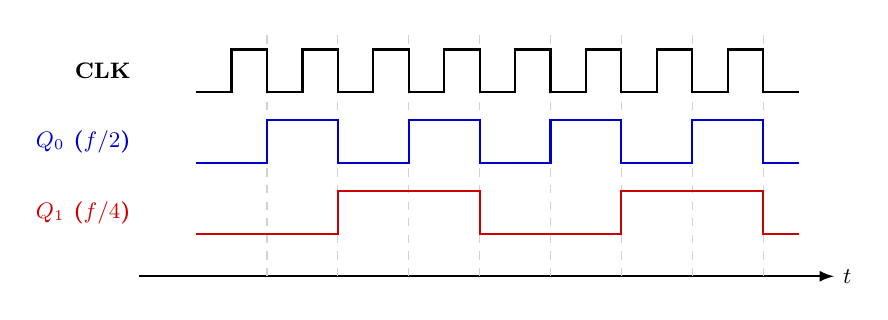
\begin{tikzpicture}[scale=0.9, every node/.style={scale=0.9}]
% Asse del tempo in basso
\draw[-latex, thick] (-0.8,-0.5) -- (9.0,-0.5) node[right, font=\small] {$t$};

% Linee verticali tratteggiate di guida
\foreach \x in {1.0, 2.0, 3.0, 4.0, 5.0, 6.0, 7.0, 8.0}{
    \draw[dashed, gray!35] (\x, -0.5) -- (\x, 3.0);
}

% CLK
\node[left, font=\small\bfseries] at (-0.8, 2.4) {CLK};
\draw[thick] (0,2.1)
\foreach \x in {0,1,2,3,4,5,6,7}{
  -- ++(0.5,0) -- ++(0,0.6) -- ++(0.5,0) -- ++(0,-0.6)
} -- ++(0.5,0);

% Q0 (f/2)
\node[left, font=\small\bfseries, color=blue!80!black] at (-0.8, 1.4) {$Q_0$ ($f/2$)};
\draw[thick, blue!80!black] (0,1.1)
\foreach \x in {0,2,4,6}{
  -- ++(1.0,0) -- ++(0,0.6) -- ++(1.0,0) -- ++(0,-0.6)
} -- ++(0.5,0);

% Q1 (f/4)
\node[left, font=\small\bfseries, color=red!80!black] at (-0.8, 0.4) {$Q_1$ ($f/4$)};
\draw[thick, red!80!black] (0,0.1)
\foreach \x in {0,4}{
  -- ++(2.0,0) -- ++(0,0.6) -- ++(2.0,0) -- ++(0,-0.6)
} -- ++(0.5,0);

\end{tikzpicture}
\end{center}

\subsection{Contatore asincrono (ripple counter)}

Nel contatore asincrono, il clock \textbf{non arriva a tutti i Flip-Flop contemporaneamente}. Solo il primo FF riceve il clock esterno; ogni FF successivo usa come proprio clock l'uscita $Q$ del FF precedente. I flip-flop sono sensibili al fronte di discesa (pallino sull'ingresso di clock) e hanno $J=K=1$ (modalità toggle): ogni FF commuta quando l'uscita del precedente passa da 1 a 0, realizzando un conteggio in avanti.

\medskip
\noindent\textcolor{teal}{\textbf{Il problema: la propagazione a catena (ripple).}} Poiché ogni FF deve aspettare che quello precedente abbia commutato, il segnale si propaga a cascata (da qui il nome \emph{ripple}). Il bit più significativo $Q_{n-1}$ non è aggiornato finché il segnale non ha attraversato tutti gli $n$ FF. Il ritardo totale vale:
\[
T_n = n \cdot T_P
\]
Questo impone che il periodo del clock sia sufficientemente lungo da permettere a tutta la catena di assestarsi prima del fronte successivo:
\[
T_{CLK} > n \cdot T_P
\]
Nei circuiti ad alta velocità questo è un limite importante: aggiungere Flip-Flop obbliga a rallentare il clock.

\begin{fitcenter}
\begin{circuitikz}[scale=0.88, every node/.style={scale=0.88}, line width=0.8pt]
\tikzset{
  jkbox/.style={
    draw, thick, minimum width=1.3cm, minimum height=1.8cm, inner sep=0pt
  }
}

% 4 Flip-Flop
\foreach \i/\x in {0/0, 1/3.2, 2/6.4, 3/9.6}{
  \node[jkbox] (B\i) at (\x, 0) {};
  % Ingressi J (in alto) e K (sotto)
  \node[font=\small\bfseries, right=2pt] at ([yshift=0.45cm]B\i.west) {$J_{\i}$};
  \node[font=\small\bfseries, right=2pt] at ([yshift=-0.05cm]B\i.west) {$K_{\i}$};
  
  % Clock negato in basso a sinistra (bubble + triangle)
  \draw ([yshift=-0.55cm]B\i.west) ++(-0.14, 0) circle (0.07cm);
  \draw ([yshift=-0.55cm]B\i.west) ++(0, 0.11) -- ++(0.16, -0.11) -- ++(-0.16, -0.11);
  \coordinate (clkpin\i) at ([yshift=-0.55cm]B\i.west);
  \coordinate (clkext\i) at ([xshift=-0.21cm, yshift=-0.55cm]B\i.west);

  % Uscita Q a destra, allineata al clock
  \node[font=\small\bfseries, left=2pt] at ([yshift=-0.55cm]B\i.east) {$Q_{\i}$};
  \coordinate (qpin\i) at ([yshift=-0.55cm]B\i.east);

  % J e K uniti insieme e salita alla barra 1
  \draw ([yshift=0.45cm]B\i.west) -- ++(-0.3, 0) coordinate (jterm\i)
     -- ([yshift=-0.05cm]B\i.west -| jterm\i) -- ([yshift=-0.05cm]B\i.west);
     
  \coordinate (midjk\i) at ($(jterm\i)!0.5!([yshift=-0.05cm]B\i.west -| jterm\i)$);
  \draw (midjk\i) -- (midjk\i |- 0, 1.45) coordinate (topconn\i);
}

% Barra orizzontale 1 in alto
\draw[thick] (-1.4, 1.45) node[left=3pt, font=\large\bfseries] {1} -- (topconn3);
\foreach \i in {0,1,2}{
  \fill (topconn\i) circle (1.5pt);
}

% Clock esterno
\draw[thick] (-0.9, -0.55) node[left, font=\small\bfseries] {CLK} -- (clkext0);

% Collegamenti a cascata: Q0 -> CLK1, Q1 -> CLK2, Q2 -> CLK3
\draw[thick] (qpin0) -- (clkext1);
\draw[thick] (qpin1) -- (clkext2);
\draw[thick] (qpin2) -- (clkext3);
\draw[-latex, thick] (qpin3) -- ++(0.7, 0);

\node[font=\small\bfseries, color=noteblue] at (4.8, -1.4) {CONTATORE ASINCRONO (RIPPLE COUNTER)};
\end{circuitikz}
\end{fitcenter}

\subsection{Contatore sincrono}

Nel contatore sincrono, il clock \textbf{arriva contemporaneamente a tutti i Flip-Flop}, eliminando il ritardo a cascata e rendendo il contatore molto più veloce.

\medskip
\noindent\textbf{Come si implementa la logica di conteggio?} Non tutti i FF devono commutare ad ogni tick: $Q_1$ deve commutare solo quando $Q_0=1$; $Q_2$ solo quando $Q_0=Q_1=1$; e così via. Questa condizione viene realizzata con \textbf{porte AND in cascata}: l'ingresso $J,K$ del FF $i$-esimo è connesso all'uscita di una porta AND che combina tutti i bit $Q_0, \ldots, Q_{i-1}$. Il FF $i$ riceve il permesso di commutare solo quando tutti i bit meno significativi valgono $1$.

\begin{fitcenter}
\begin{circuitikz}[scale=0.88, every node/.style={scale=0.88}, line width=0.8pt]
\tikzset{
  jkbox/.style={
    draw, thick, minimum width=1.3cm, minimum height=1.8cm, inner sep=0pt
  }
}

% 4 Flip-Flop
\foreach \i/\x in {0/0, 1/3.4, 2/7.0, 3/10.6}{
  \node[jkbox] (B\i) at (\x, 0) {};
  % Ingressi K (in alto) e J (sotto)
  \node[font=\small\bfseries, right=2pt] at ([yshift=0.45cm]B\i.west) {$K_{\i}$};
  \node[font=\small\bfseries, right=2pt] at ([yshift=-0.05cm]B\i.west) {$J_{\i}$};
  
  % Clock negato in basso a sinistra (bubble + triangle)
  \draw ([yshift=-0.55cm]B\i.west) ++(-0.14, 0) circle (0.07cm);
  \draw ([yshift=-0.55cm]B\i.west) ++(0, 0.11) -- ++(0.16, -0.11) -- ++(-0.16, -0.11);
  \coordinate (clkpin\i) at ([yshift=-0.55cm]B\i.west);
  \coordinate (clkext\i) at ([xshift=-0.21cm, yshift=-0.55cm]B\i.west);
  \coordinate (clktap\i) at ([xshift=-0.40cm, yshift=-0.55cm]B\i.west);

  % Uscita Q a destra
  \node[font=\small\bfseries, left=2pt] at ([yshift=-0.55cm]B\i.east) {$Q_{\i}$};
  \coordinate (qpin\i) at ([yshift=-0.55cm]B\i.east);

  % K e J uniti
  \coordinate (kterm\i) at ([xshift=-0.35cm, yshift=0.45cm]B\i.west);
  \coordinate (jterm\i) at ([xshift=-0.35cm, yshift=-0.05cm]B\i.west);
  \draw ([yshift=0.45cm]B\i.west) -- (kterm\i);
  \draw ([yshift=-0.05cm]B\i.west) -- (jterm\i);
}

% FF0: K0 e J0 collegati al livello logico 1
\draw[thick] (kterm0) -- (jterm0);
\draw[thick] ($(kterm0)!0.5!(jterm0)$) -- ++(-0.35, 0) -- ++(0, 0.8) node[above, font=\large\bfseries] {1};

% FF1: Q0 va al tratto verticale di K1-J1 che sale sopra FF1 verso AND1
\coordinate (vert1) at (kterm1);
\draw[thick] (qpin0) -- (qpin0 -| vert1) -- (jterm1) node[circle, fill, inner sep=1.1pt]{} -- (kterm1) node[circle, fill, inner sep=1.1pt]{} -- ([yshift=0.9cm]kterm1) coordinate (topFF1);

% AND1 tra FF1 e FF2
\node[and port, scale=0.65] (AND1) at (5.3, 0.45) {};
\draw[thick] (topFF1) -- (topFF1 -| AND1.in 1) -- (AND1.in 1);
\draw[thick] (qpin1) -- (qpin1 -| AND1.in 2) -- (AND1.in 2);

% Uscita AND1 va al tratto verticale di K2-J2 che sale sopra FF2 verso AND2
\coordinate (vert2) at (kterm2);
\draw[thick] (AND1.out) -- (vert2) node[circle, fill, inner sep=1.2pt]{} -- (jterm2);
\draw[thick] (vert2) -- ([yshift=0.9cm]kterm2) coordinate (topFF2);

% AND2 tra FF2 e FF3
\node[and port, scale=0.65] (AND2) at (8.9, 0.45) {};
\draw[thick] (topFF2) -- (topFF2 -| AND2.in 1) -- (AND2.in 1);
\draw[thick] (qpin2) -- (qpin2 -| AND2.in 2) -- (AND2.in 2);

% Uscita AND2 va a K3-J3 di FF3
\coordinate (vert3) at (kterm3);
\draw[thick] (AND2.out) -- (vert3) node[circle, fill, inner sep=1.2pt]{} -- (jterm3);

% Uscita Q3 finale
\draw[-latex, thick] (qpin3) -- ++(0.7, 0);

% Bus CLK comune in basso
\coordinate (clkbus_y) at (0, -1.2);
\draw[thick] (-1.6, -1.2) node[left=2pt, font=\small\bfseries] {CLK} -- (11.4, -1.2);
\foreach \i in {0,1,2,3}{
  \draw[thick] (clkext\i) -- (clktap\i) |- (clktap\i |- clkbus_y) node[circle, fill, inner sep=1.2pt]{};
}

\node[font=\small\bfseries, color=noteblue] at (5.3, -1.7) {CONTATORE SINCRONO};
\end{circuitikz}
\end{fitcenter}

\subsection{Azzeramento dopo un certo conteggio (contatore modulo-M)}

Spesso non si vuole un contatore che vada da $0$ a $2^n-1$, ma che si fermi ad un numero specifico $M$ e poi riparta da zero.

\medskip
\noindent\textbf{Implementazione:} si aggiunge una porta AND ai cui ingressi arrivano le uscite $Q_i$ che sono a $1$ nella rappresentazione binaria di $M$. Non appena il contatore raggiunge $M$, l'uscita della porta AND va a $1$ e genera un segnale di \textbf{RESET asincrono} che azzera immediatamente tutti i FF riportandoli a $Q=0000$.

\medskip
\noindent\textbf{Attenzione al glitch sull'ultimo conteggio:} il valore $M$ compare realmente in uscita per un brevissimo istante (il tempo necessario affinché la porta AND lo riconosca e il reset arrivi) prima che tutto sia azzerato. L'ultimo stato ha quindi una durata anomala:
\[
T_{\text{stato }M} = T_f(\text{JK-FF}) + T_P(\text{AND})
\]

\medskip
\begin{esercizio}{Esempio: azzeramento dopo il numero 5 (bastano 3 bit)}
Quando $Q_3 Q_2 Q_1 Q_0 = 0101_2$ (valore 5), la porta AND sottostante rileva questa condizione (alimentata da $Q_0$ e $Q_2$, gli unici bit a 1 di $5=101_2$) e genera il segnale di \textbf{RESET asincrono di tutti i FF}, che vengono azzerati attraverso i loro ingressi di clear.\\[0.3em]
Il contatore percorre quindi gli stati $0, 1, 2, 3, 4$, ciascuno per un periodo di clock, mentre lo stato 5 compare solo per il brevissimo tempo $T_f(\text{JK-FF}) + T_P(\text{AND})$ necessario all'azzeramento. Il ciclo dura 5 periodi di clock: si tratta di un \textbf{contatore modulo-5} (divisore per 5). Per ottenere un modulo-$M$ con reset asincrono si decodifica quindi il valore $M$ stesso.
\end{esercizio}

\begin{fitcenter}
\begin{circuitikz}[scale=0.88, every node/.style={scale=0.88}, line width=0.8pt]
\tikzset{
  jkbox/.style={
    draw, thick, minimum width=1.3cm, minimum height=1.8cm, inner sep=0pt
  }
}

% 4 Flip-Flop
\foreach \i/\x in {0/0, 1/3.4, 2/7.0, 3/10.6}{
  \node[jkbox] (B\i) at (\x, 0) {};
  \node[font=\small\bfseries, right=2pt] at ([yshift=0.45cm]B\i.west) {$K_{\i}$};
  \node[font=\small\bfseries, right=2pt] at ([yshift=-0.05cm]B\i.west) {$J_{\i}$};
  
  % Clock negato in basso a sinistra
  \draw ([yshift=-0.55cm]B\i.west) ++(-0.14, 0) circle (0.07cm);
  \draw ([yshift=-0.55cm]B\i.west) ++(0, 0.11) -- ++(0.16, -0.11) -- ++(-0.16, -0.11);
  \coordinate (clkpin\i) at ([yshift=-0.55cm]B\i.west);
  \coordinate (clkext\i) at ([xshift=-0.21cm, yshift=-0.55cm]B\i.west);
  \coordinate (clktap\i) at ([xshift=-0.40cm, yshift=-0.55cm]B\i.west);

  % Uscita Q a destra
  \node[font=\small\bfseries, left=2pt] at ([yshift=-0.55cm]B\i.east) {$Q_{\i}$};
  \coordinate (qpin\i) at ([yshift=-0.55cm]B\i.east);

  % K e J uniti
  \coordinate (kterm\i) at ([xshift=-0.35cm, yshift=0.45cm]B\i.west);
  \coordinate (jterm\i) at ([xshift=-0.35cm, yshift=-0.05cm]B\i.west);
  \draw ([yshift=0.45cm]B\i.west) -- (kterm\i);
  \draw ([yshift=-0.05cm]B\i.west) -- (jterm\i);
}

% FF0: K0 e J0 collegati a 1
\draw[thick] (kterm0) -- (jterm0);
\draw[thick] ($(kterm0)!0.5!(jterm0)$) -- ++(-0.35, 0) -- ++(0, 0.8) node[above, font=\large\bfseries] {1};

% FF1: Q0 va al tratto verticale di K1-J1 che sale sopra FF1 verso AND1
\coordinate (vert1) at (kterm1);
\draw[thick] (qpin0) -- (qpin0 -| vert1) -- (jterm1) node[circle, fill, inner sep=1.1pt]{} -- (kterm1) node[circle, fill, inner sep=1.1pt]{} -- ([yshift=0.9cm]kterm1) coordinate (topFF1);

% AND1 tra FF1 e FF2
\node[and port, scale=0.65] (AND1) at (5.3, 0.45) {};
\draw[thick] (topFF1) -- (topFF1 -| AND1.in 1) -- (AND1.in 1);
\draw[thick] (qpin1) -- (qpin1 -| AND1.in 2) -- (AND1.in 2);

% Uscita AND1 va al tratto verticale di K2-J2 che sale sopra FF2 verso AND2
\coordinate (vert2) at (kterm2);
\draw[thick] (AND1.out) -- (vert2) node[circle, fill, inner sep=1.2pt]{} -- (jterm2);
\draw[thick] (vert2) -- ([yshift=0.9cm]kterm2) coordinate (topFF2);

% AND2 tra FF2 e FF3
\node[and port, scale=0.65] (AND2) at (8.9, 0.45) {};
\draw[thick] (topFF2) -- (topFF2 -| AND2.in 1) -- (AND2.in 1);
\draw[thick] (qpin2) -- (qpin2 -| AND2.in 2) -- (AND2.in 2);

% Uscita AND2 va a K3-J3 di FF3
\coordinate (vert3) at (kterm3);
\draw[thick] (AND2.out) -- (vert3) node[circle, fill, inner sep=1.2pt]{} -- (jterm3);

% Uscita Q3 finale
\draw[-latex, thick] (qpin3) -- ++(0.7, 0);

% Bus CLK comune in basso
\coordinate (clkbus_y) at (0, -1.2);
\draw[thick] (-1.6, -1.2) node[left=2pt, font=\small\bfseries] {CLK} -- (11.4, -1.2);
\foreach \i in {0,1,2,3}{
  \draw[thick] (clkext\i) -- (clktap\i) |- (clktap\i |- clkbus_y) node[circle, fill, inner sep=1.2pt]{};
}

% Logica di RESET ASINCRONO: in 1 ancorato esattamente sotto Q2
\node[and port, scale=0.75, anchor=in 1] (AND_RST) at (qpin2 |- 0, -2.0) {};

% Linea da Q0 verso l'AND di reset (in basso)
\fill[gray!60!black] (1.6, -0.55) circle (1.3pt);
\draw[thick, gray!60!black] (1.6, -0.55) |- (AND_RST.in 2);

% Linea da Q2 verso l'AND di reset (scende diritta da Q2 direttamente nell'ingresso 1)
\fill[gray!60!black] (qpin2) circle (1.3pt);
\draw[thick, gray!60!black] (qpin2) -- (AND_RST.in 1);

% Uscita Reset sotto FF3
\draw[thick, gray!60!black] (AND_RST.out) -- ++(0.3, 0) node[right, font=\footnotesize\bfseries, text=gray!60!black] {RESET ASINCRONO DI TUTTI I FF};

\end{circuitikz}
\end{fitcenter}

\clearpage
\subsection{Ripple Carry Output (RCO)}

I contatori binari integrati (come il classico \textbf{SN74LS163A}) includono un'uscita speciale chiamata \textbf{RCO} (Ripple Carry Output).

\medskip
\noindent\textbf{A cosa serve?} Quando si collegano più chip in cascata per formare un contatore a più bit (es. 8, 12, 16 bit), ogni chip deve segnalare al successivo quando ha terminato il proprio ciclo di conteggio. Il chip delle unità segnala al chip delle decine; il chip delle decine segnala a quello delle centinaia; e così via.

L'RCO è l'uscita di una porta NOR con 5 ingressi (i 4 $\overline{Q_i}$ e il segnale di \emph{enable} $T$ negato, cioè $\text{RCO}=T\cdot Q_AQ_BQ_CQ_D$): va a $1$ per esattamente \textbf{un periodo di clock} quando il contatore ha raggiunto il valore massimo (tipicamente $Q=1111=15$). Solo in quel preciso istante tutti i $\overline{Q_i}$ sono a $0$, e la NOR dà $1$:
\[
\text{RCO} = 1 \quad \text{per un periodo } T_{CLK} \text{ quando il conteggio è al massimo.}
\]

\noindent Il chip successivo nella catena usa questo impulso RCO come \emph{enable} (o come clock) per incrementare il proprio conteggio: in questo modo si realizzano contatori a 8, 12, 16 bit collegando semplicemente chip da 4 bit in cascata tramite RCO.

\begin{center}
\begin{tikzpicture}[scale=0.75, every node/.style={scale=0.75}]
% Corpo integrato
\draw[thick, fill=blue!3] (0,0) rectangle (5.0, 5.8);
\node[font=\large\bfseries, color=noteblue] at (2.5, 5.25) {SN74LS163A};
\node[font=\scriptsize, color=gray] at (2.5, 4.85) {Contatore sincrono a 4 bit};

% Ingressi di controllo (sinistra alto)
\foreach \y/\lab in {4.3/CLK, 3.7/$\overline{\text{CLR}}$, 3.1/$\overline{\text{LOAD}}$, 2.5/ENP, 1.9/ENT}{
  \draw[-latex, thick] (-1.2, \y) node[left, font=\small\bfseries]{\lab} -- (0, \y);
}

% Ingressi dati paralleli (sinistra basso)
\foreach \y/\lab in {1.3/A, 0.95/B, 0.6/C, 0.25/D}{
  \draw[-latex] (-1.2, \y) node[left, font=\footnotesize]{DATA \lab} -- (0, \y);
}

% Uscite dati (destra)
\foreach \y/\lab in {4.3/$Q_A$, 3.5/$Q_B$, 2.7/$Q_C$, 1.9/$Q_D$}{
  \draw[-latex, thick] (5.0, \y) -- (6.2, \y) node[right, font=\small\bfseries]{\lab};
}

% Uscita RCO (destra basso)
\draw[-latex, thick, color=noteblue] (5.0, 0.9) -- (6.2, 0.9) node[right, font=\small\bfseries]{RCO};
\node[left, font=\scriptsize, color=gray] at (5.0, 0.9) {Carry};

\end{tikzpicture}
\end{center}

% ======================================================================
\section*{Riepilogo del Capitolo}

\begin{important}
I registri a scorrimento spostano dati attraverso una catena di Flip-Flop D in quattro modalità (\textbf{SISO, SIPO, PISO, PIPO}), mentre i contatori avanzano di stato a ogni colpo di clock in forma \textbf{asincrona} (ripple, più lenta) o \textbf{sincrona} (AND in cascata, senza ritardo di propagazione cumulato).
\end{important}

\begin{note}
\textbf{Formule fondamentali:}
\begin{itemize}
    \item \textbf{Vincolo di temporizzazione:} $T_P > T_H$, $\; T_S + T_P < T_{CLK}$ (setup/hold/propagazione).
    \item \textbf{Modalità di scorrimento:} SISO, SIPO, PISO, PIPO.
    \item \textbf{Ritardo del contatore asincrono (ripple) a $n$ bit:} $T_n = n\cdot T_P$, quindi $T_{CLK} > n\cdot T_P$.
    \item \textbf{Contatore sincrono:} porte AND in cascata su $Q_0,\dots,Q_{i-1}$ abilitano il toggle del Flip-Flop $i$-esimo, eliminando il ritardo cumulato.
    \item \textbf{Contatore modulo-$M$:} decodifica dello stato $M$ tramite AND $\to$ reset asincrono di tutti i Flip-Flop.
\end{itemize}
\end{note}

